%\chapter{Results}
\chapter{Planing}

%\section{Experiment 1}
\section{Risk Analysis}
Risk analysis is critical to a successful project, exotically for inexperienced younger researchers doing an MSc. dissertation. The following risk register lists 10 hazards and actions to avoid or decrease the impact. 

\begin{table}[ht]
\scriptsize
\begin{tabular}{@{}|l|l|c|c|c|l|@{}}
\toprule
\multicolumn{1}{|c|}{\textbf{}} & \multicolumn{1}{c|}{\textbf{Hazard/Impact}}                                                                                                                & \textbf{L} & \textbf{I} & \textbf{E} & \multicolumn{1}{c|}{\textbf{Action}}                                                                                                \\ \midrule
1                                  & \begin{tabular}[c]{@{}l@{}}not understand the requirements and constraints/ \\ may cost huge time in wrong direction\end{tabular}                           & 2                   & 4               & 4                  & \begin{tabular}[c]{@{}l@{}}do more literature survey;\\ discuss with the supervisor timely;\end{tabular}                            \\ \midrule
2                                  & \begin{tabular}[c]{@{}l@{}}incomplete or unworkable plan/\\ may cause low efficiency in implementation \\ or unable to achieve expected result\end{tabular} & 3                   & 4               & 4                  & \begin{tabular}[c]{@{}l@{}}revisit key tasks and task dependencies; \\ update work plan timely;\end{tabular}                        \\ \midrule
3                                  & \begin{tabular}[c]{@{}l@{}}unable to meet the supervisor/\\ may not get suggestions and feedback on time\end{tabular}                                       & 1                   & 2               & 1                  & \begin{tabular}[c]{@{}l@{}}book appointment in advance; \\ contact via email;\end{tabular}                                          \\ \midrule
4                                  & \begin{tabular}[c]{@{}l@{}}unrealistic schedule/\\ may delay the project\end{tabular}                                                                       & 2                   & 3               & 3                  & \begin{tabular}[c]{@{}l@{}}detailed schedule estimation; \\ workable milestones; \\ incremental development;\end{tabular}           \\ \midrule
5                                  & \begin{tabular}[c]{@{}l@{}}poor time management;\\ may delay the project \\ and affect the quality of the research\end{tabular}                             & 4                   & 4               & 4                  & \begin{tabular}[c]{@{}l@{}}detailed work plan; \\ check backlogs on weekly basis; \\ write monthly reflection;\end{tabular}         \\ \midrule
6                                  & \begin{tabular}[c]{@{}l@{}}accidentally loss work or codes/\\ may cost huge time in restoration\end{tabular}                                                & 1                   & 2               & 1                  & \begin{tabular}[c]{@{}l@{}}version control; \\ multiple local back-up;\end{tabular}                                                 \\ \midrule
7                                  & \begin{tabular}[c]{@{}l@{}}lack of knowledge on a certain topic/\\ may delay a deadline \\ and even fail the project\end{tabular}                           & 3                   & 4               & 4                  & \begin{tabular}[c]{@{}l@{}}take time to read literature; \\ keep notes; \\ seek help from teachers;\end{tabular}                    \\ \midrule
8                                  & \begin{tabular}[c]{@{}l@{}}lack of experience on software/\\ may delay a deadline \\ or block the project\end{tabular}                                      & 2                   & 3               & 3                  & \begin{tabular}[c]{@{}l@{}}take time to study online tutorials; \\ learning by practicing; \\ seek help from teachers;\end{tabular} \\ \midrule
9                                  & \begin{tabular}[c]{@{}l@{}}lack of experience on programming; \\ may delay a deadline\end{tabular}                                                          & 2                   & 2               & 3                  & \begin{tabular}[c]{@{}l@{}}learning by practicing; \\ have clear practice plan;\end{tabular}                                        \\ \midrule
10                                 & \begin{tabular}[c]{@{}l@{}}lack of experience in doing research/\\ may delay deadlines \\ and affect the quality of the research\end{tabular}               & 4                   & 3               & 4                  & \begin{tabular}[c]{@{}l@{}}read reference books; \\ write sub-task reports; \\ consult the supervisor;\end{tabular}                 \\ \bottomrule
\end{tabular}
\caption{A risk register; Columns of L, I and E stand for likelihood, impact and exposure respectively.}
\label{tab:risk}
\end{table}



%\lipsum  % Replace with your text

%\section{Experiment 2}
\section{Work Plan}

This project is divided into 3 stages: theoretical framework, experiment implementation and project dissertation. The Gantt chart below (Figure \ref{fig:gantt}) show the timeline, sub-tasks, milestones and dependencies between tasks. For a good project organisation, stage retrospectives and a experiment journal will also be written.

\begin{figure}[ht]
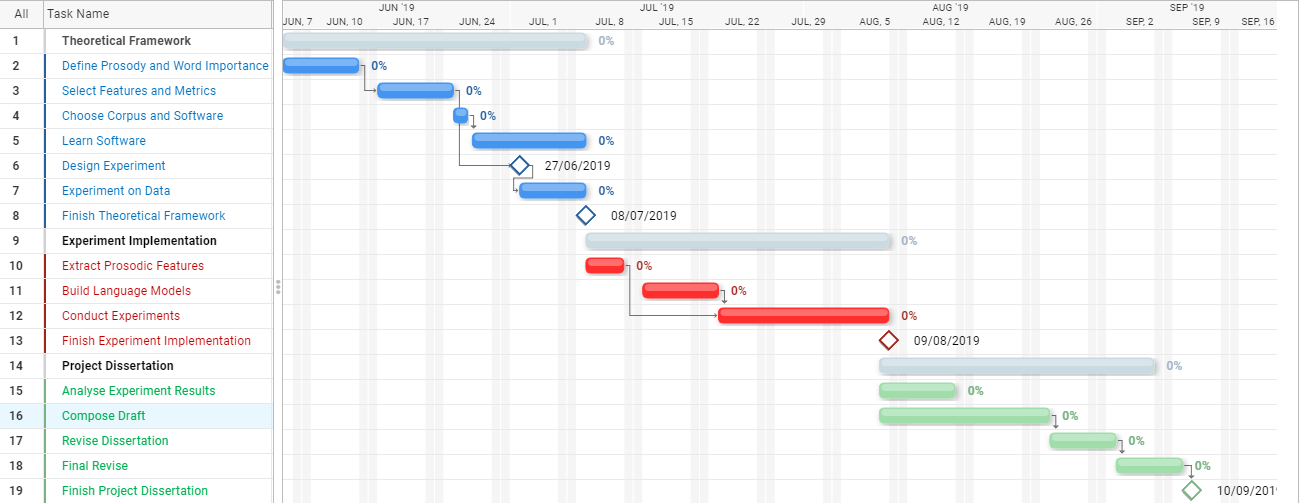
\includegraphics[width=15cm]{figures/gantt.png}
\caption{A Gantt chart of project plan}
\label{fig:gantt}
\end{figure}

%\lipsum  % Replace with your text
